%& -shell-escape
\documentclass{article}
\usepackage[utf8]{inputenc}
\usepackage{xcolor}
\usepackage{graphicx}
\usepackage{colortbl}
\usepackage{rotating}
\usepackage{multirow}
\usepackage{multicol}
\usepackage{booktabs}
\usepackage{bigstrut}
\usepackage{listings}
\usepackage{python}
\graphicspath{{images/}}


\definecolor{codegreen}{rgb}{0,0.6,0}
\definecolor{codegray}{rgb}{0.5,0.5,0.5}
\definecolor{codepurple}{rgb}{0.58,0,0.82}
\definecolor{backcolour}{rgb}{0.95,0.95,0.92}

\lstdefinestyle{mystyle}{
    backgroundcolor=\color{backcolour},   
    commentstyle=\color{codegreen},
    keywordstyle=\color{magenta},
    numberstyle=\tiny\color{codegray},
    stringstyle=\color{codepurple},
    basicstyle=\ttfamily\footnotesize,
    breakatwhitespace=false,         
    breaklines=true,                 
    captionpos=b,                    
    keepspaces=true,                 
    numbers=left,                    
    numbersep=5pt,                  
    showspaces=false,                
    showstringspaces=false,
    showtabs=false,                  
    tabsize=2
}
\lstset{style=mystyle}

\title{Bilgisayar Mühendisliğinde Matematik Uygulamaları}
\author{Mert ATAY - 180202090}
\date{25 Mayıs 2021}

\begin{document}

\maketitle
\paragraph{
  Programlama Dili : Python
  \newline
  Kullanılan Kütüphaneler : Pandas, Numpy, Scikit-learn, Seaborn 
}
\section{Örnek 1:}
\subsection{Problemimizin Tanımı:}



\hspace{1cm}Bu örnekteki problemimizde herhangi bir üniversiteye başvuru yapan öğrenci adayların üniversite yönetimi tarafından kabul edilip edilmeyeceğini belirlemek için logistik regresyon analizi yöntemiyle sonuç elde edilmek isteniyor.


\subsection{Problemde Uygulanan Adımlar}

\hspace{1cm} Bu problemimizde uygulanacak adımları sırasıyla veri seti oluşturulup, kodda çözüm içi neler yaptığımızla devam edip, en son olarak programımızın sonuçlarını göstereceğim.



\subsubsection{1.Adım : Veri Seti Oluşturma}
\hspace{1cm}Öncelikle binary classfication yapısına göre burada iki olası sonuç vardır:
Ya "admitted"(1 değeri) olarak veya  "rejected"(0 değeri) olarak sonuçlanacaktır.
\newline

Eğer Python'da bir lojistik regresyon oluşturmak istersek burada:
\begin{itemize}
    \item Bağımlı değişken, bir kişinin kabul edilip edilmeyeceğini temsil eder,
    \item Bağımsız değişkenlerimiz ise GMAT puanı, GPA ve iş deneyimi süresidir.
\end{itemize}

Veri setini aşağıda görebilirsiniz:

\begin{table}
    \centering
    \begin{tabular}{|l|l|l|l|l|}
    \hline
         & gmat & gpa & work\_experience & admitted \\ \hline
        0 & 780 & 4 & 3 & 1 \\ \hline
        1 & 750 & 3.9 & 4 & 1 \\ \hline
        2 & 690 & 3.3 & 3 & 0 \\ \hline
        3 & 710 & 3.7 & 5 & 1 \\ \hline
        4 & 680 & 3.9 & 4 & 0 \\ \hline
        5 & 730 & 3.7 & 6 & 1 \\ \hline
        6 & 690 & 2.3 & 1 & 0 \\ \hline
        7 & 720 & 3.3 & 4 & 1 \\ \hline
        8 & 740 & 3.3 & 5 & 1 \\ \hline
        9 & 690 & 1.7 & 1 & 0 \\ \hline
        10 & 610 & 2.7 & 3 & 0 \\ \hline
        11 & 690 & 3.7 & 5 & 1 \\ \hline
        12 & 710 & 3.7 & 6 & 1 \\ \hline
        13 & 680 & 3.3 & 4 & 0 \\ \hline
        14 & 770 & 3.3 & 3 & 1 \\ \hline
        15 & 610 & 3 & 1 & 0 \\ \hline
        16 & 580 & 2.7 & 4 & 0 \\ \hline
        17 & 650 & 3.7 & 6 & 1 \\ \hline
        18 & 540 & 2.7 & 2 & 0 \\ \hline
        19 & 590 & 2.3 & 3 & 0 \\ \hline
        20 & 620 & 3.3 & 2 & 1 \\ \hline
        21 & 600 & 2 & 1 & 0 \\ \hline
        22 & 550 & 2.3 & 4 & 0 \\ \hline
        23 & 550 & 2.7 & 1 & 0 \\ \hline
        24 & 570 & 3 & 2 & 0 \\ \hline
        25 & 670 & 3.3 & 6 & 1 \\ \hline
        26 & 660 & 3.7 & 4 & 1 \\ \hline
        27 & 580 & 2.3 & 2 & 0 \\ \hline
        28 & 650 & 3.7 & 6 & 1 \\ \hline
        29 & 660 & 3.3 & 5 & 1 \\ \hline
        30 & 640 & 3 & 1 & 0 \\ \hline
        31 & 620 & 2.7 & 2 & 0 \\ \hline
        32 & 660 & 4 & 4 & 1 \\ \hline
        33 & 660 & 3.3 & 6 & 1 \\ \hline
        34 & 680 & 3.3 & 5 & 1 \\ \hline
        35 & 650 & 2.3 & 1 & 0 \\ \hline
        36 & 670 & 2.7 & 2 & 0 \\ \hline
        37 & 580 & 3.3 & 1 & 0 \\ \hline
        38 & 590 & 1.7 & 4 & 0 \\ \hline
        39 & 690 & 3.7 & 5 & 1 \\ \hline
    \end{tabular}
\end{table}

\newpage

Bu veri setiyle çalıştım. Kodda ise nasıl oluşturulduğunu görebilirsiniz:

\begin{lstlisting}[language=Python, caption=Veri Seti Oluşturma]
import pandas as pd
from sklearn.model_selection import train_test_split
from sklearn.linear_model import LogisticRegression
from sklearn import metrics
import seaborn as sn
import matplotlib.pyplot as plt

#veri setini excel dosyasindan okuyoruz
dataset = pd.read_excel('dataset.xlsx',index_col=0)
#veri setini dataframe olacak sekilde pandas kut. yardimiyla tanimliyoruz.
df = pd.DataFrame(dataset)
#Dataframe i gosteriyoruz
print (df)
\end{lstlisting}


Sonuç olarak da aşağıya bu terminal sonucu gelecektir:
\begin{figure}[htp]
    \centering
    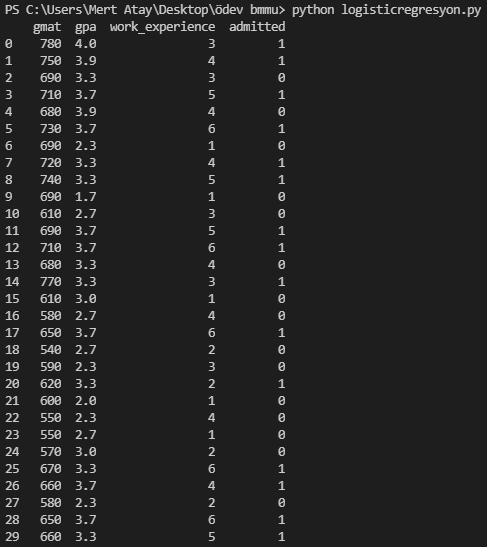
\includegraphics[width=10cm]{1.png}
    \caption{Veri Seti Oluşturma (Sonucu)}
    \label{fig:galaxy}
\end{figure}

\newpage

\subsubsection{2.Adım: Logistic Regresyon Modeli}
\hspace{1cm}2.adımda modelimizi oluşturan kodları  ve onların sonuçlarını göreceksiniz.\\
Öncelikle analiz için x ve y değerlerimizin olması gerekiyor. Bunları şu şekilde aldım.

\begin{lstlisting}[language=Python, caption=x ve y Değerleri]
X = df[['gmat', 'gpa','work_experience']]
y = df['admitted']
\end{lstlisting}

Daha sonra bu değerlerden eğitilecek verileri ayrı ve test verileri ayrı olacak şekilde seçtim.

\begin{lstlisting}[language=Python, caption=Kullanılacak verilerin ayrıştırılması]
#egitilecek x degerlerinden bir test veri seti elde ediyoruz. Belirtilen test_size = veri
#setinin ceyregini kullaniyor.
X_train,X_test,y_train,y_test = train_test_split(X,y,test_size=0.25,random_state=0)
\end{lstlisting}

\par Şimdi modelimizi oluşturabilecek kıvama geldi. Modelimizin ismini logisticregression değişkenine tanımlayarak model oluşturuldu.Daha sonra eğilecek değerler verildi ve en son da tahmin (predict) işlemleri yapıldı.

\begin{lstlisting}[language=Python, caption=Logistic Regression]
#lojistik regresyon modelini belirtiyoruz
logistic_regression= LogisticRegression()
#analize giricek modeli eğitiyoruz
logistic_regression.fit(X_train,y_train)
#yukarıdan alınan x elemanlarından oluşan test verisetinden eğitilen ve 
#tahmin edilen y değerlerini değişkene atıyoruz
y_pred=logistic_regression.predict(X_test)
print("------------------------")
print (X_test) 
print("------------------------")
print (y_pred)
\end{lstlisting}
Eğer örnek bir veri seti görmek istersek :

\begin{figure}[htp]
    \centering
    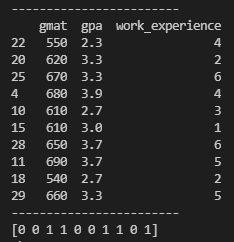
\includegraphics[width=6cm, height=4cm]{3.png}
    \caption{Test Verileri}
    \label{fig:my_label}
\end{figure}
\newpage
Bu verilerde test amaçlı olarak kullanılıp eğitilen modele göre bir doğruluk payı değeri alırlar. Bu değerin 0 ile 1 arasında olması gerekir. Bu değer 0'a ne kadar çok yaklaşırsa tahminler olumsuz sonuçlar ortaya çıkaracaktır. Fakat 1'e ne kadar çok yaklaşırsa bir o kadar olumlu sonuç ortaya çıkma şansı doğurur. Yukarıda gördüğünüz örnek verilerde bir dizide bulunan 0 ve 1 değerleri gördünüz. Test verilerinde kabul edilen sayısı ve kabul edilmeyenler eğitilen modele göre bu sonucu almıştır.\par Son olarak bu doğruluk değeri ve eğitilen modelimizin doğruluk değerini görelim.
\subsubsection{3.Adım: Sonuçlar}
\begin{lstlisting}[language=Python, caption=Logistic Regression Sonuç Bastırımı]
print("Skor:" + str(logistic_regression.score(X_train,y_train)))
print("------------------------")
print('Doğruluğu: ',metrics.accuracy_score(y_test, y_pred)) #Doğruluk skoru
print("------------------------")



confusion_matrix = pd.crosstab(y_test, y_pred, rownames=['Gercek'], colnames=['Tahmin'])
sn.heatmap(confusion_matrix, annot=True)

plt.show()#Ekranda goster
\end{lstlisting}
\begin{figure}
    \centering
    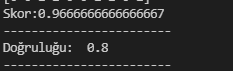
\includegraphics{4.png}
    \caption{Skor ve Doğruluk Değeri}
    \label{fig:my_label}
\end{figure}

Şimdiki sonuçta gerçek ve tahmin  değerleri arasındaki 4 farklı şekilde bulunan:
\begin{itemize}
    \item Doğru Pozitifler: 4
    \item Doğru Negatifler: 4
    \item Yanlış Pozitifler : 1
    \item Yanlış Negaifler : 1
\end{itemize}

şeklide elde edilmiştir.

\begin{figure}[htp]
    \centering
    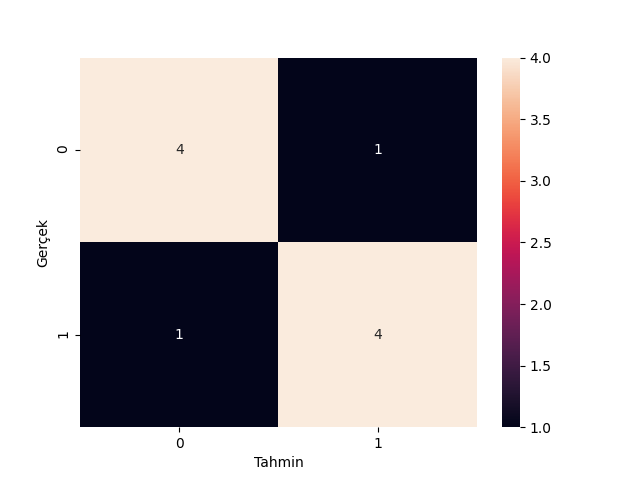
\includegraphics{sonuç_grafiği.png}
    \caption{Sonuç Grafiği}
    \label{fig:my_label}
\end{figure}

\newpage

\section{Örnek 2:}

\subsection{Problemimizin Tanımı:}

\hspace{1cm}Bu örnekteki problemimizde herhangi bir araba galerisinde bulunan arabaların katettiği yolun km olarak arabanın değerine göre hangi durumda olduğunu anlamak için lineer regresyon analizi yöntemiyle sonuç elde edilmek isteniyor.

\subsection{Problemde Uygulanan Adımlar}

\hspace{1cm} Aynı şekilde bu problemimizde uygulanacak adımları sırasıyla veri seti oluşturulup, kodda çözüm içi neler yaptığımızla devam edip, en son olarak programımızın sonuçlarını göstereceğim.

\subsubsection{1.Adım : Veri Seti Oluşturma}
\hspace{1cm} Lineer regresyonda, bir dizi noktaya en uygun düz çizgiyi veya hiper düzlemi bulmak için kullanılmakta idi. Bir diğer ifadeyle lineer regresyon, en uygun düz çizgi (regresyon çizgisi) kullanarak bağımlı değişken (Y) ile bir veya daha fazla bağımsız değişken (X) arasında bir ilişki kurar. Aşağıdaki grafikte kırmızı çizgi en uygun düz çizgi olarak adlandırılır.\par
Ben de bu veri setinde arabaların kilometre ömürlerine göre fiyatlarının nasıl bir ilişki içerisinde olacağını göstereceğim.\par
Hadi veri setimizi görelim:
\begin{center}
    
    
    \begin{tabular}{|l|l|l|}
    
    \hline
        Km & Yil & Fiyat \\ \hline
        69000 & 6 & 18000 \\ \hline
        35000 & 3 & 34000 \\ \hline
        57000 & 5 & 26100 \\ \hline
        22500 & 2 & 40000 \\ \hline
        46000 & 4 & 31500 \\ \hline
        59000 & 5 & 26750 \\ \hline
        52000 & 5 & 32000 \\ \hline
        72000 & 6 & 19300 \\ \hline
        91000 & 8 & 12000 \\ \hline
        67000 & 6 & 22000 \\ \hline
        83000 & 7 & 18700 \\ \hline
        79000 & 7 & 19500 \\ \hline
        59000 & 5 & 26000 \\ \hline
        58780 & 4 & 27500 \\ \hline
        82450 & 7 & 19400 \\ \hline
        25400 & 3 & 35000 \\ \hline
        28000 & 2 & 35500 \\ \hline
        69000 & 5 & 19700 \\ \hline
        87600 & 8 & 12800 \\ \hline
        52000 & 5 & 28200 \\ \hline
    \end{tabular}
    
\end{center}
\newpage

Bu veri setiyle çalıştım. Kodda ise nasıl oluşturulduğunu görebilirsiniz:

\begin{lstlisting}[language=Python, caption=Veri Seti Oluşturma]
import numpy as np
import matplotlib.pyplot as plt 
import pandas as pd
from sklearn.linear_model import LinearRegression

data = pd.read_csv('fiyatlar.csv')  # veriyi aliyoruz
X = data.iloc[:, 0].values.reshape(-1, 1)  # Verideki degerleri numpy dizisine donduruyoruz
Y = data.iloc[:, 2].values.reshape(-1, 1)  # -1, satirlarin boyutunun hesaplandigi, ancak 1 sutun oldugu anlamina gelir
print("----------------------------")
print(data)
\end{lstlisting}
Sonuç olarak da aşağıya bu terminal sonucu gelecektir:
\begin{figure}[htp]
    \centering
    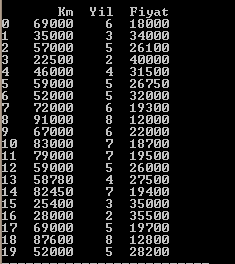
\includegraphics{liR_1.png}
    \caption{Veri Seti}
    \label{fig:my_label}
\end{figure}

\subsubsection{2.Adım: Lineer Regresyon Modeli}
\hspace{1cm}2.adımda modelimizi oluşturan kodları  ve onların sonuçlarını göreceksiniz.\\
Öncelikle analiz için x ve y değerlerimizin olması gerekiyor. Bunları şu şekilde aldım.

\begin{lstlisting}[language=Python, caption=x ve y Değerleri]
X = data.iloc[:, 0].values.reshape(-1, 1)  # Verideki degerleri numpy dizisine donduruyoruz
Y = data.iloc[:, 2].values.reshape(-1, 1)  # -1, satirlarin boyutunun hesaplandigi, ancak 1 sutun oldugu anlamina gelir
\end{lstlisting}

Daha sonra bu değerleri kullanan eğitim modelimizi oluşturdum.

\begin{lstlisting}[language=Python, caption=Model]
linear_regressor = LinearRegression()  # model objemizi olusturduk
linear_regressor.fit(X, Y)  # lineer regresyon modelimizi egittik
Y_pred = linear_regressor.predict(X)  # tahminler yaptik
print(X)#eğittiğimiz x değerleri
print("--------------------------")
print(Y_pred)#tahminler
\end{lstlisting}
\begin{multline}
    Şimdi modelimizi oluşturduk. Modelimizi lineerregressor değişkenine tanımladık. Daha sonra eğilecek değerler verildi ve en son da tahmin (predict) işlemleri yapıldı. Bu işlemlerin sonucunda galeride bulunan arabaların km ömürlerine göre fiyatlarının ne seviyede olduğunu ilişkilendirmeye çalıştım. En son da bu değerleri görelim.
\end{multline}
    



\begin{figure}[htp]
    \centering
    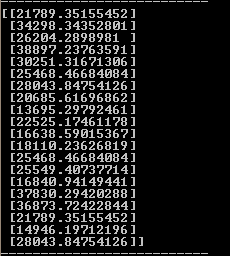
\includegraphics{liR_2.png}
    \caption{Tahmin değerleri}
    \label{fig:my_label}
\end{figure}

\begin{figure}[htp]
    \centering
    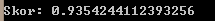
\includegraphics{liR_3.png}
    \caption{Doğruluk Skoru}
    \label{fig:my_label}
\end{figure}

\subsubsection{3.Adım: Sonuçlar}
\begin{lstlisting}[language=Python, caption=Lineer Regression Sonuç Bastırımı]
print("Skor: " + str(linear_regressor.score(X,Y)))

plt.xlabel("Km ler")
plt.ylabel("Tahmini fiyatlar")
plt.scatter(X, Y)#x ve y değerlerine göre noktalarımızı grafiğe yerleştirdik.
plt.plot(X, Y_pred, color='red')
plt.show()
\end{lstlisting}

Sonuç grafiğini de aşağıda görebilirsiniz.

\begin{figure}[htp]
    \centering
    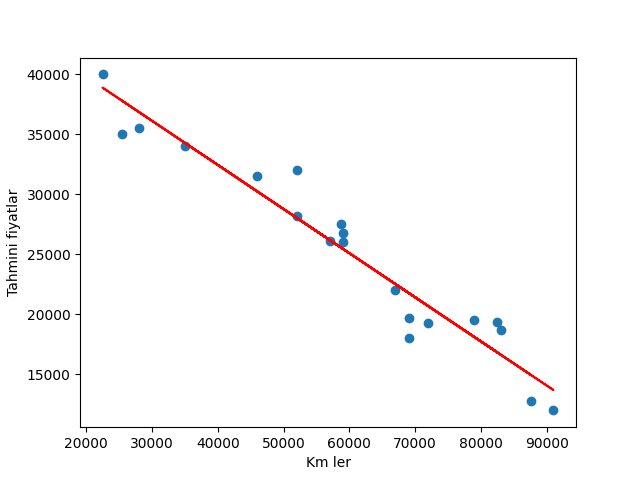
\includegraphics{liR_sonuc.png}
    \caption{Sonuç Grafiği}
    \label{fig:my_label}
\end{figure}








\end{document}
